\clearpage % clear the prior chapter's page

\chapter{ConfChangeMover: Integrative modeling of conformational changes in LeuT-fold transporters using sparse spectroscopy data} \label{app:confchangemover}
%\vspace{-7mm}
%\bigskip

This Appendix is based on unpublished data.

%\vspace{-7mm}
\bigskip

\section{Introduction}

Active transporters, such as those with the LeuT-fold, undergo conformational changes to import and export substrates into and out of the cell \citep*{Kazmier2017}. Canonical models of symport and antiport mandate that these proteins adopt several different conformers. However, their structures are often experimentally resolved in one specific state, leaving scientists guessing at the the molecular drivers of substrate translocation. Sparse experimental data, collected using techniques such as \gls{epr} \citep*{Jeschke2012, Kazmier2014a} and/or \gls{hdxms} \citep*{Merkle2018}, can report on the structural basis of alternating access when higher-resolution methods such as \gls{cryoem} and X-ray crystallography fail. In conjunction with computational modeling, these data can provide a glimpse of the molecular details of these unknown conformers. Nonetheless, the sparseness and ambiguity of these experimental restraints make it challenging to model structures that are consistent with the data provided while retaining atomic-detail information provided by the starting X-ray or \gls{cryoem} structure.

We reasoned that the general problem surrounding the accurate modeling of conformational changes is similar in principle to that of structure refinement, in which the atomic details of structural models are deduced from low-quality models \citep*{Heo2019, Park2019, Read2019}. Recent advancements in \gls{mc} refinement methods have relied on conservative sampling described as "broken-chain kinematics" \citep*{Park2018}, in which rigid-body segments of structural models are manipulated in isolation and rejoined using loop closure (see section \ref{sec:loophash_intro} for a more detailed discussion on protein loop closure methods). This strategy has been instrumental to recent advances in homology modeling and is the foundation of widely-used methods including RosettaCM \citep*{Song2013} and Modeller \citep*{Eswar2006}. However, \gls{mc} methods are rarely employed for conformational change modeling problems, which have instead generally been tackled using either gradient minimization \cite*{Evans2020} or \gls{md} simulations \citep*{Marinelli2019, Sfriso2016}. Both methods are computationally expensive and can potentially understate the extent to which protein backbones reconfigure. 

Here we describe a general-purpose \gls{mc} sampling method, ConfChangeMover, which we implemented in the macromolecular modeling program Rosetta \citep*{Leaver-fay2011, Leman2020} and designed to model conformational changes using sparse experimental data (Figure \ref{fig:ccm_scheme}). The method combines recent conceptual advances borrowed from cutting-edge homology modeling methods with novel sampling approaches designed to conservatively manipulate a starting structure. Whereas homology modeling is concerned with identifying the dihedral angles of a protein that satisfy spatial restraints provided by one or more template models, our approach instead samples spatial rearrangements consistent with dihedral angles observed in the starting structure. We first demonstrate ConfChangeMover on a panel of soluble proteins using simulated $\mathrm{C_{\upalpha}}$-$\mathrm{C_{\upalpha}}$ distance restraints. Then, using experimental \gls{epr} data that has been previously published, we apply the method to three transporters with the LeuT-fold fold (described in detail in Chapter \ref{ch:leutintro}).


\begin{figure}[h]
\centering
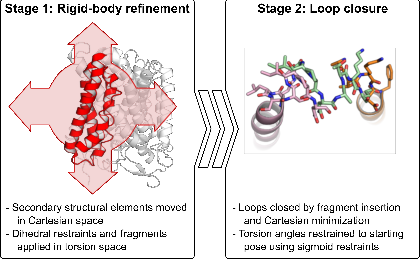
\includegraphics[width=5in]{Figures/ccm_scheme.pdf}
 \caption[Overview of the ConfChangeMover sampler.]{Overview of the ConfChangeMover sampler.}
\label{fig:ccm_scheme}
\end{figure}


\section{Materials and Methods}

\subsection{Overview of the sampling approach}


ConfChangeMover was implemented in Rosetta and executed in RosettaScripts \citep*{Fleishman2011}. As with RosettaCM, it samples candidate structural models using a two-stage strategy (Figure \ref{fig:ccm_scheme}). Prior to the first stage, the input structure is converted to a coarse-grained model with side chains replaced by immobile centroid pseudo-atoms. Cutpoints are introduced at residues located on loops connecting pairs of rigid bodies, or segments, which consist of either $\mathrm{\upalpha}$-helices or $\mathrm{\upbeta}$-sheets identified using the \gls{dssp} \citep*{Kabsch1983}. These cutpoints allow the positions and conformations of these segments to be perturbed either in isolation or in concert in the first stage without downstream propagation to rest of the protein via the "lever-arm effect" \citep*{Tyka2012}. A series of sigmoid dihedral constraints, discussed below in section \ref{sec:confchangemover_restraints}, are added to model.

During the first stage, several types of perturbations are randomly introduced in the structural model. These include:

\begin{itemize}
    \item \textbf{Rigid-body movements of one \gls{sse}.} Rotation angles and translation vectors are randomly drawn from normal distributions with standard deviations of 15° and \SI{2.0}{\angstrom}, respectively.
    \item \textbf{Rigid-body movements of multiple spatially adjacent \gls{sse}s.} The number of \gls{sse}s randomly ranges from 2 to $N-1$, where $N$ is the number of segments in the model, and the movement parameters match those used for a single \gls{sse}.
    \item \textbf{Helical twists.} Helices are twisted by a randomly chosen angle drawn from a normal distribution with a standard deviation of 15°.
    \item \textbf{Fragment insertion.} The dihedral angles of a three-residue stretch of the protein are modified to match those of a randomly chosen sequence fragment obtained from the PDB. Fragments were obtained using the Robetta web server as previously described \citep*{Kim2004}.
\end{itemize}

Throughout this stage, \gls{sse}s that are adjacent in sequence are constrained such that their N- and C-terminal ends can be plausibly bridged by the loop connecting them. We achieved this by automatically rejecting moves that separate the termini of consecutive \gls{sse}s by distances greater than $2.65n_{\mathup{res}}+2.11$ \AA, where $n_{\mathup{res}}$ is the number of residues in the loop \citep*{Woetzel2012}.

During the second stage, loops are closed using a method similar to one described previously \citep*{Rohl2004} that is used by RosettaCM \citep*{Song2013}. However, ConfChangeMover supplements this procedure using stretches of the starting model ranging from three to fifteen residues in length. The perturbations available include:

\begin{itemize}
    \item \textbf{Fragment superimposition over gap regions.} Nine-residue fragments obtained from the PDB are superimposed over unresolved gaps in the structure.
    \item \textbf{Fragment superimposition over randomly chosen regions.} Nine-residue fragments are superimposed over randomly-chosen regions, which can include those that do not contain chainbreaks.
    \item \textbf{Template superimposition.} Stretches of residues with lengths ranging from nine to fifteen residues are copied from the starting conformation and superimposed over the model.
\end{itemize}

As with RosettaCM, during the final 25\% of the second stage, each move is followed by a brief Cartesian minimization \citep*{Conway2014} using the limited-memory Broyden-Fletcher-Goldfarb-Shanno algorithm \citep*{Byrd1995}. At the end of stage 2, the entire model is minimized using the same approach.

During an optional third stage, all-atom side chains replace the centroid pseudo-atoms, and the entire model is iteratively minimized as previously described \citep*{Conway2014, Song2013}.

\subsection{Application of constraints during modeling}\label{sec:confchangemover_restraints}

Several types of constraints are applied to these models throughout the algorithm. To account for the relative invariance of protein dihedral angles during conformational change modeling (see section \ref{sec:ccm_results_dihedrals}), circular sigmoidal restraints are added to the $\phi$ and $\psi$ angles of the model based on either the starting conformation or a separate model provided by the user:

\begin{equation}
    S_{\upphi}(x) = \left( 1 + \exp \left( | \phi_{\mathup{sim}} - \phi_{\mathup{exp}} | - \frac{\pi}{2} \right) \right)^{-1} + \left( 1 + \exp \left( | \phi_{\mathup{sim}} - \phi_{\mathup{exp}} | + \frac{\pi}{2} \right) \right)^{-1}
\end{equation}

\begin{equation}
    S_{\uppsi}(x) = \left( 1 + \exp \left( | \psi_{\mathup{sim}} - \psi_{\mathup{exp}} | - \frac{\pi}{2} \right) \right)^{-1} + \left( 1 + \exp \left( | \psi_{\mathup{sim}} - \psi_{\mathup{exp}} | + \frac{\pi}{2} \right) \right)^{-1}
\end{equation}

Additionally, following stage 1, coordinate constraints were applied to the $\mathrm{C_{\upalpha}}$ atoms of all residues belonging to \gls{sse}s. This allowed fragment insertions during stage 2 to close loops while minimally affecting the dihedral angles obtained following stage 1.

\subsection{Benchmark on soluble proteins using simulated distance restraints}

We first tested ConfChangeMover on seven soluble proteins (Table \ref{tab:ccm_proteins}). These topologically dissimilar proteins were selected from previous benchmarks \citep*{Jeschke2012, Sfriso2016}. We first modeled all missing residues using RosettaCM \citep*{Song2013}. Distance restraints between $\mathrm{C_{\upalpha}}$ atoms were selected from the starting structure using a modification of the Zheng-Brooks algorithm as implemented in the program MMM \citep*{Jeschke2012, Jeschke2018a, Polyhach2011, Zheng2005}, with one restraint per twenty residues in the total protein sequence, rounding up. For the benchmark on soluble proteins, we compared ConfChangeMover to fragment insertion, in which the dihedral angles of the starting structures were directly modified. For both methods, regions that did not undergo conformational transitions between the two states were not permitted to move and were not used for \gls{rmsd} calculations.

\begin{table}[h]
\scriptsize
\renewcommand{\tabcolsep}{0.09cm}
\centering
\caption[Protein structures used in the benchmark of ConfChangeMover.]{Protein structures used in the benchmark of ConfChangeMover. $^{\dagger}$ A model of \gls{of} vSGLT was generated from the X-ray structure of the homolog SiaT. This model was not used as a target model in this benchmark. $^{\ddagger}$ Insufficient experimental restraints were available to model the \gls{of}-to-\gls{if} transition in LeuT.}

%\newcolumntype{Y}{>{\raggedright\arraybackslash}X}

% Structures are marked if they were mutated ($\dagger$) or bound to inhibitors ($\ddagger$) or antibodies ($\mathsection$).}

\begin{center}
\begin{tabular}{l l l l r}
\toprule \\
\textbf{Protein \emph{(Organism)}} & \textbf{PDB A (Resolution)} & \textbf{PDB B (Resolution)} & \textbf{Length} & \textbf{References} \\
\midrule \\
\multicolumn{5}{l}{\textbf{Soluble proteins (simulated data)}} \\
Adenosylcobinamide kinase (\emph{Salmonella enterica}) & 1CBU (\SI{2.30}{\angstrom}) & 1C9K (\SI{2.20}{\angstrom}) & 181 & \citep*{Thompson1998, Thompson1998a} \\
DNA polymerase I (\emph{Thermophilus aquaticus}) &  2KTQ (\SI{2.30}{\angstrom}) & 3KTQ (\SI{2.30}{\angstrom}) & 832 & \citep*{Li1998} \\
Glutamine-binding protein (\emph{Escherichia coli}) & 1GGG (\SI{2.30}{\angstrom}) & 1WDN (\SI{1.94}{\angstrom}) & 248 & \citep*{Hsaio1996, Sun1998} \\
Lactoferrin (\emph{Homo sapiens}) & 1LFH (\SI{2.80}{\angstrom}) & 1LFG (\SI{2.20}{\angstrom}) & 710 & \citep*{Haridas1995, Norris1991} \\
Leucine-binding protein (\emph{E. coli}) & 1USI (\SI{1.80}{\angstrom}) & 1USG (\SI{1.53}{\angstrom}) & 369 & \citep*{Magnusson2004} \\
Mitochondrial aspartate aminotransferase (\emph{Gallus gallus}) & 1AMA (\SI{2.30}{\angstrom}) & 9AAT (\SI{2.20}{\angstrom}) & 423 & \citep*{McPhalen1992, McPhalen1992a} \\
Pol alpha DNA polymerase (\emph{Escherichia} phage RB69) & 1IG9 (\SI{2.60}{\angstrom}) & 1IH7 (\SI{2.21}{\angstrom}) & 903 & \citep*{Franklin2001} \\
\\
\multicolumn{5}{l}{\textbf{LeuT-fold proteins (experimental data)}} \\
LeuT (\emph{Aquifex aeolicus}) & 2A65 (\SI{1.65}{\angstrom}) & $\mathrm{3TT3}^\ddagger$ (\SI{3.22}{\angstrom}) & 513 & \citep*{Krishnamurthy2012, Yamashita2005} \\
Mhp1 (\emph{Microbacterium tumefaciens}) & 2JLN (\SI{2.85}{\angstrom}) & 2X79 (\SI{3.80}{\angstrom}) & 489 & \citep*{Shimamura2010, Weyand2008} \\
vSGLT (\emph{Vibrio parahaemolyticus}) & 2XQ2 (\SI{2.73}{\angstrom}) & $\mathrm{5NV9^\dagger}$ (\SI{1.95}{\angstrom}) & 543 & \citep*{Wahlgren2018, Watanabe2010} \\
\bottomrule \\
\end{tabular} 
\end{center}
\label{tab:ccm_proteins}
\end{table}

\subsection{Benchmark on LeuT-fold transporters proteins using experimental EPR restraints}

For the benchmark using experimental data, ConfChangeMover was tested using three LeuT-fold transporter proteins: LeuT \citep*{Krishnamurthy2012, Yamashita2005}, Mhp1 \citep*{Shimamura2010, Weyand2008}, and vSGLT \citep*{Watanabe2010} (Table \ref{tab:ccm_proteins}). These three proteins have previously been studied using \gls{epr}, and all undergo ligand-dependent conformational transitions between \gls{if} and \gls{of} conformations \citep*{Claxton2010, Kazmier2014, Kazmier2014a, Paz2018}.

Four transitions of interest were used to benchmark ConfChangeMover (Table \ref{tab:ccm_proteins}). In each case, experimental data was provided using the RosettaDEER module (see Chapter \ref{ch:rosettadeer}). For LeuT, the \gls{if}-to-\gls{of} transition took advantage of distance restraints collected on LeuT in the presence of the detergent $\mathrm{\upbeta}$-OG \citep*{Kazmier2014a}. In Mhp1, the \gls{of}-to-\gls{if} and \gls{if}-to-\gls{of} transitions were simulated using \gls{deer} data collected either without substrates or with both sodium and benzylhydantoin, respectively \citep*{Kazmier2014}. Finally, because vSGLT has only been crystallized in \gls{if} conformations \citep*{Faham2008, Watanabe2010}, we modeled the \gls{of}-to-\gls{if} transition by starting from a previously published \gls{of} homology model generated from the homologous sialic acid transporter SiaT \citep*{Paz2018, Wahlgren2018}. The \gls{if}-to-\gls{of} transition of vSGLT and the \gls{of}-to-\gls{if} transition of LeuT were not modeled.

For both benchmarks, we set stages 1 and 2 to consist of 50,000 rounds and 1,000 rounds, respectively. The weights of the score terms \emph{dihedral\_constraint}, \emph{atompair\_constraint}, and \emph{coordinate\_constraint} were set to 1.0, 10.0, and 1.0, respectively. The Rosetta scoring functions \emph{score3} and \emph{score4\_smooth\_cart} were used for stages 1 and 2, respectively. We generated 100 models using each method for the soluble protein benchmark and 1000 models for the LeuT-fold benchmark. 

\section{Results and Discussion}

\subsection{Most dihedral angles do not change during conformational isomerization}\label{sec:ccm_results_dihedrals}

To determine the extent to which dihedral $\phi$ and $\psi$ angles rotate during conformational change, we compared pairs of structures from a panel of conformational changes used in a recent benchmark \citep*{Jeschke2012a}. Comparison of proteins in multiple states revealed that the overwhelming majority of backbone dihedral angles in proteins remain unchanged when undergoing conformational transitions, suggesting that interconversion between two states may be facilitated by a small fraction of residues as previously suggested \citep*{Sauer2020} (Figure \ref{fig:ccm_angles}). This expectation was implemented as a modeling restraint using circular sigmoidal functions on the backbone $\phi$ and $\psi$ angles (see section \ref{sec:confchangemover_restraints}). Sigmoidal restraints have previously been used for modeling proteins using restraints with a small number of false positives, such as those obtained using residue coevolution \citep*{Ovchinnikov2015, Ovchinnikov2017, Teixeira2017}, because they favor structural models that satisfy as many restraints as possible while minimizing the contribution of noisy data to the resulting model. 

\begin{figure}[h]
\centering
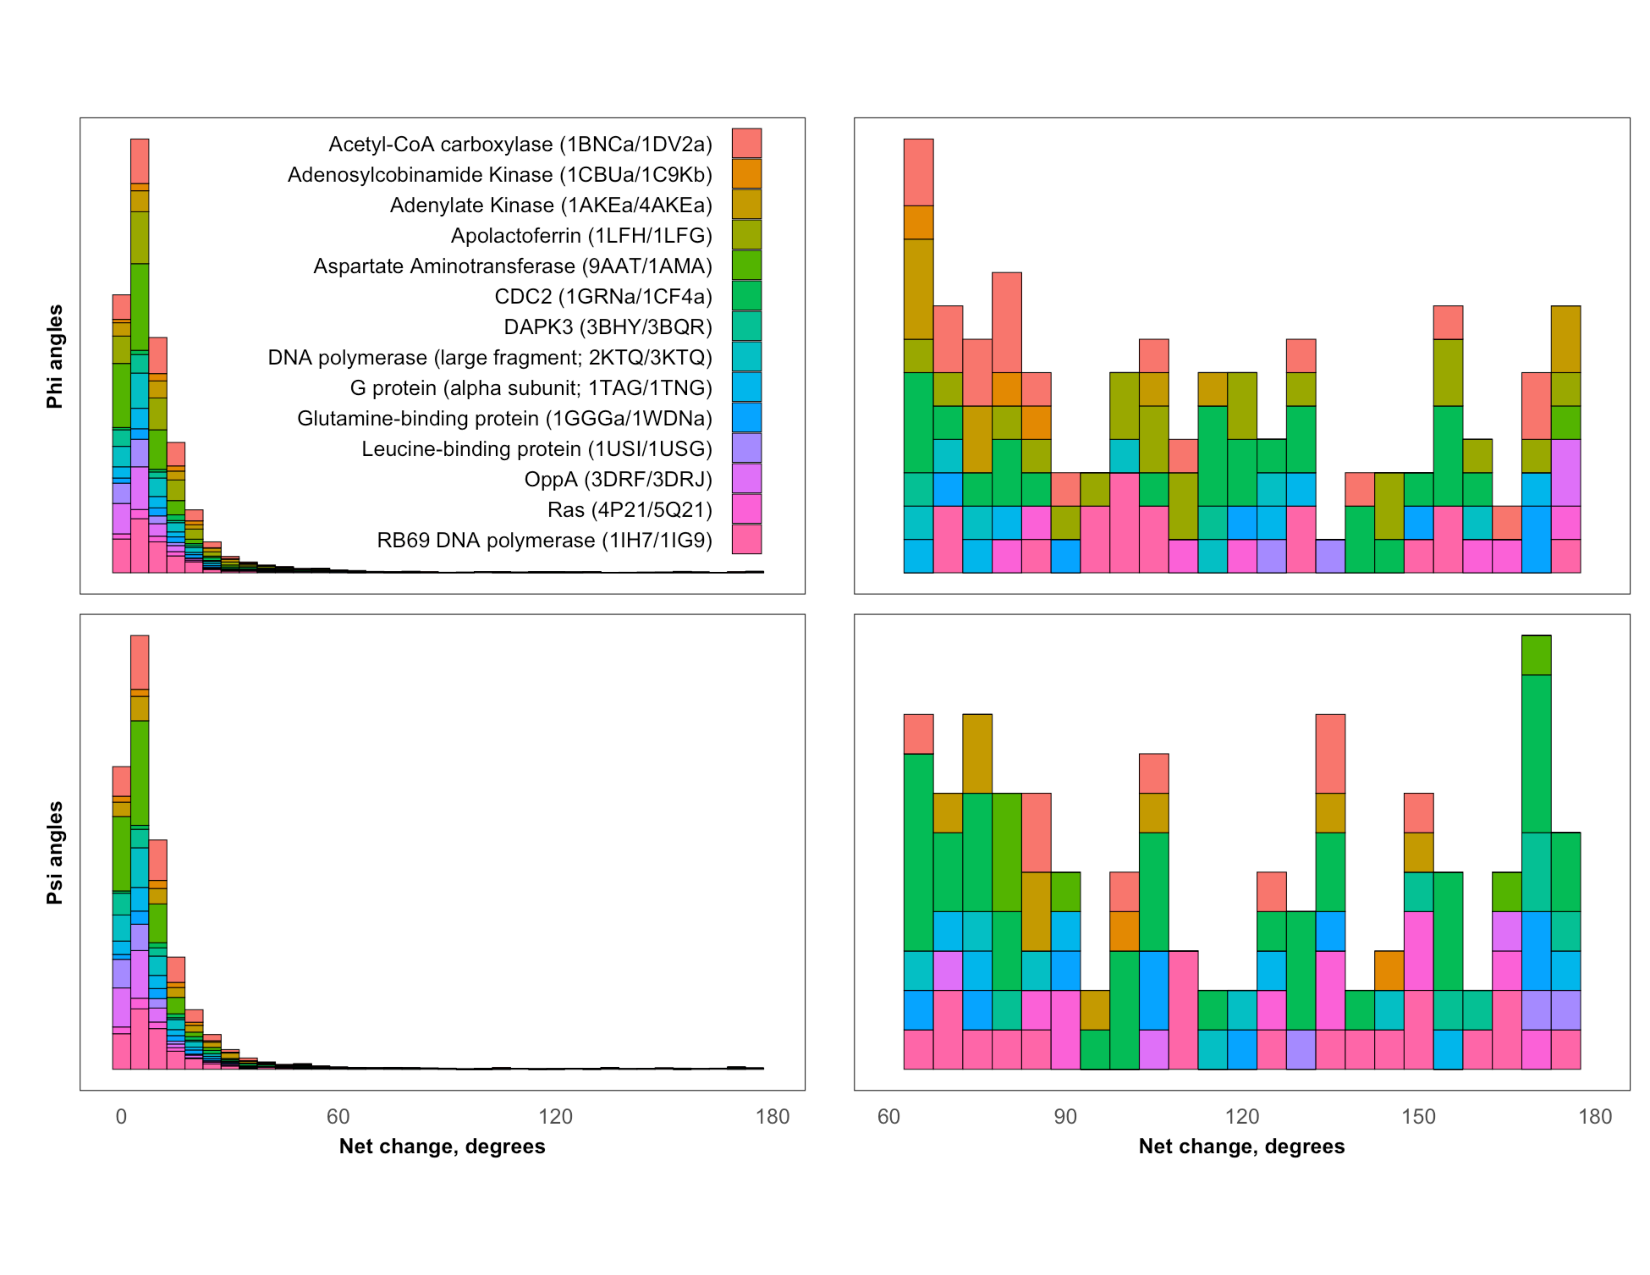
\includegraphics[width=6.5in]{Figures/ccm_angles.pdf}
 \caption[Rotational changes observed in the dihedral angles of various proteins undergoing conformational changes.]{Rotational changes observed in the dihedral angles observed in various proteins undergoing conformational changes. Left: the overwhelming majority of dihedral angles in the dataset rotate less than 30° during isomerization. Right: Close-up of cases that rotate more than 60°.}
\label{fig:ccm_angles}
\end{figure}

\subsection{Benchmark on soluble proteins}

We first benchmarked ConfChangeMover on a panel of seven soluble proteins using simulated distance restraints (Table \ref{tab:ccm_proteins}). Both directions were used as part of the benchmark, leading to fourteen total transitions. These proteins were specifically chosen for their complex modes of conformational isomerization, wherein loops and \gls{sse}s moves in ways that are unlikely to be easily recapitulated by simple rotation of backbone dihedral angles \citep*{Dastvan2016a, Krug2016}. To test that this was the case, the performance of ConfChangeMover was compared to simple fragment insertion. For both methods, regions that do not move in between these two states were not manipulated. Distance restraints between $\mathrm{C_{\upalpha}}$ atoms were chosen using a previously published restraint-picking algorithm \citep*{Jeschke2012a, Zheng2005} and simulated from the target structure. Following the simulation, $\mathrm{C_{\upalpha}}$ \gls{rmsd} values were calculated exclusively from the mobile regions of the protein.

The results are plotted in Figure \ref{fig:ccm_soluble}. In the absence of restraints, the majority of models sampled using ConfChangeMover were nearly identical to the starting model, indicated by the dashed line, suggesting that the starting structure generally occupied an energy minimum that may be difficult to escape. Introducing simulated $\mathrm{C_{\upalpha}}$-$\mathrm{C_{\upalpha}}$ restraints led to improvements in \gls{rmsd} in every protein except lactoferrin.  In contrast, using restraints with fragment insertion generally led to unfolding of the models and worsening of \gls{rmsd} relative to the starting structure (see Figure \ref{fig:ccm_soluble}.A), despite the fact that fragments were only inserted in stretches of mobile residues. In general, the breadth of models sampled this way was both far larger and universally poorer in quality than those obtained ConfChangeMover. The exception to this second point, lactoferrin, appeared to be modeled relatively easily by simple changes in the dihedral angles connecting two domains. Additionally, the majority of simulated restraints obtained using the modified Zheng-Brookes restraint-picking algorithm discussed above did not cover mobile portions of the protein. As a result, we believe the aggressive sampling available to fragment insertion may have been beneficial to escaping the local minimum and sampling conformers similar to the target. Nevertheless, the majority of models did worsen in \gls{rmsd} relative to the starting structure.

\begin{figure}[h!]
\centering
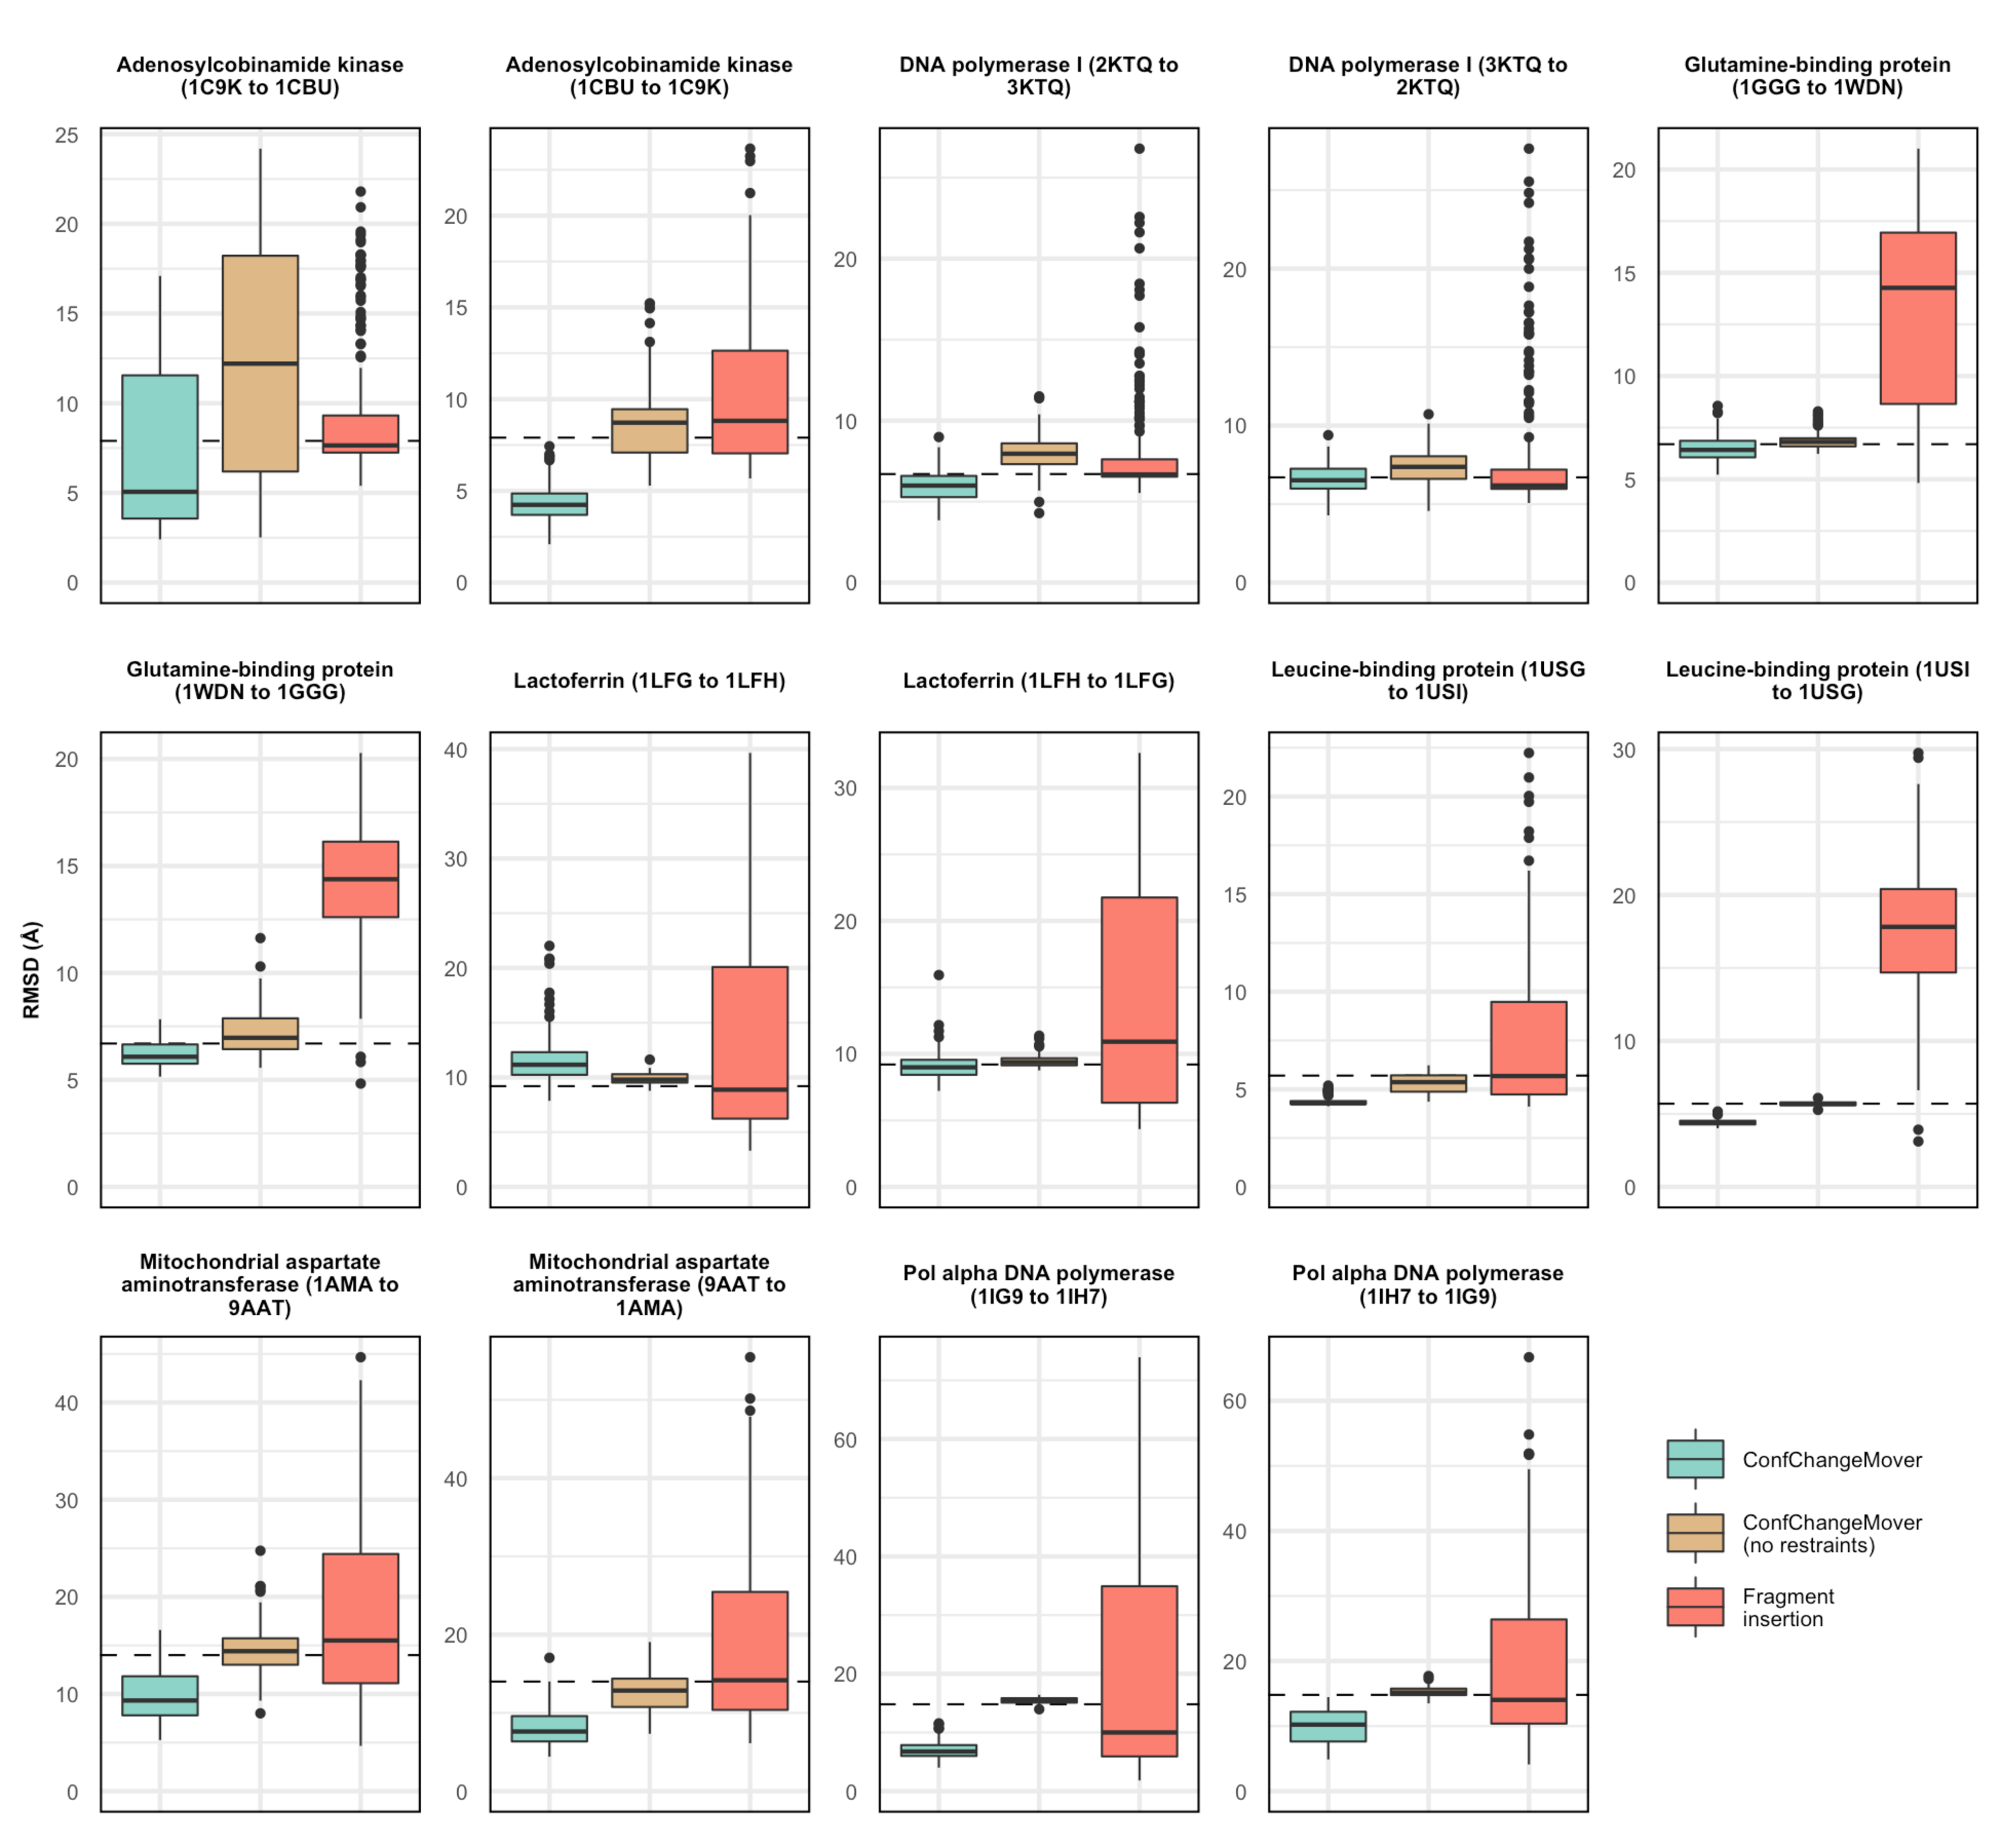
\includegraphics[width=6.5in]{Figures/ccm_soluble.pdf}
 \caption[ConfChangeMover outperforms fragment insertion in Rosetta when modeling conformational changes in soluble proteins using simulated $\mathrm{C_{\upalpha}}$ restraints.]{ConfChangeMover outperforms fragment insertion in Rosetta when modeling conformational changes in soluble proteins using simulated $\mathrm{C_{\upalpha}}$ restraints. Starting models indicated by the dashed black line. }
\label{fig:ccm_soluble}
\end{figure}

The remaining proteins in the benchmark set generally show a consistent pattern in which sampling using ConfChangeMover is focused and worsening of models is generally avoided. This is the principal challenge of structure refinement \citep*{Park2018}, as there are many more ways to ruin a structural model than improve it.

\subsection{Benchmark on LeuT-fold transporters using experimental data}

With these results in hand, we then applied this method to LeuT-fold transporters that have been experimentally studied using \gls{epr}. The transmembrane domains of these transporters are entirely $\mathrm{\upalpha}$-helical and undergo various divergent modes of isomerization to facilitate translocation of substrates across the membrane (see Chapter \ref{ch:leutintro} for details). Libraries of \gls{deer} measurements collected in LeuT, Mhp1, and vSGLT are generally consistent with experimental structures. For LeuT, due to outstanding controversies surrounding the conformational details of the \gls{if} state \citep*{Kazmier2014a, Sohail2016}, we exclusively simulated the \gls{if}-to-\gls{of} transition using experimental measurements collected in the detergent \gls{bog}. Helices in the bundle domain, as well as \gls{tmh}5 and \gls{el}4, were permitted to move, while the positions of the hash domain and \gls{tmh}10-12 were fixed. For Mhp1, both the \gls{if} and \gls{of} conformations were largely found to be consistent with \gls{epr} data collected in the apo and substrate-bound state and indicated rigid-body movement of the hash domain and bending of \gls{tmh}5. For vSGLT, which has only been crystallized in \gls{if} conformations, we modeled the \gls{of}-to-\gls{if} conformational change starting from an \gls{of} homology model generated from the structure of the homolog SiaT \citep*{Wahlgren2018} that was generated for a previous study \citep*{Paz2018}. The conformational changes suggested by the \gls{epr} data are largely consistent with those expected from this model and suggest a mechanism of alternating access that combines elements of both LeuT and Mhp1 that involve helices across the whole protein. We repeated the conformational change modeling procedure and compared it to both fragment insertion and to the homology modeling program RosettaCM \citep*{Song2013}. Additionally, to evaluate the impact of experimental restraints on modeling, ConfChangeMover was also run with simulated \gls{deer} restraints generated using MDDS \citep*{Islam2013}, as well as simulated $\mathrm{C_{\upalpha}}$-$\mathrm{C_{\upalpha}}$ distance restraints generated from the target model.


\begin{figure}[h!]
\centering
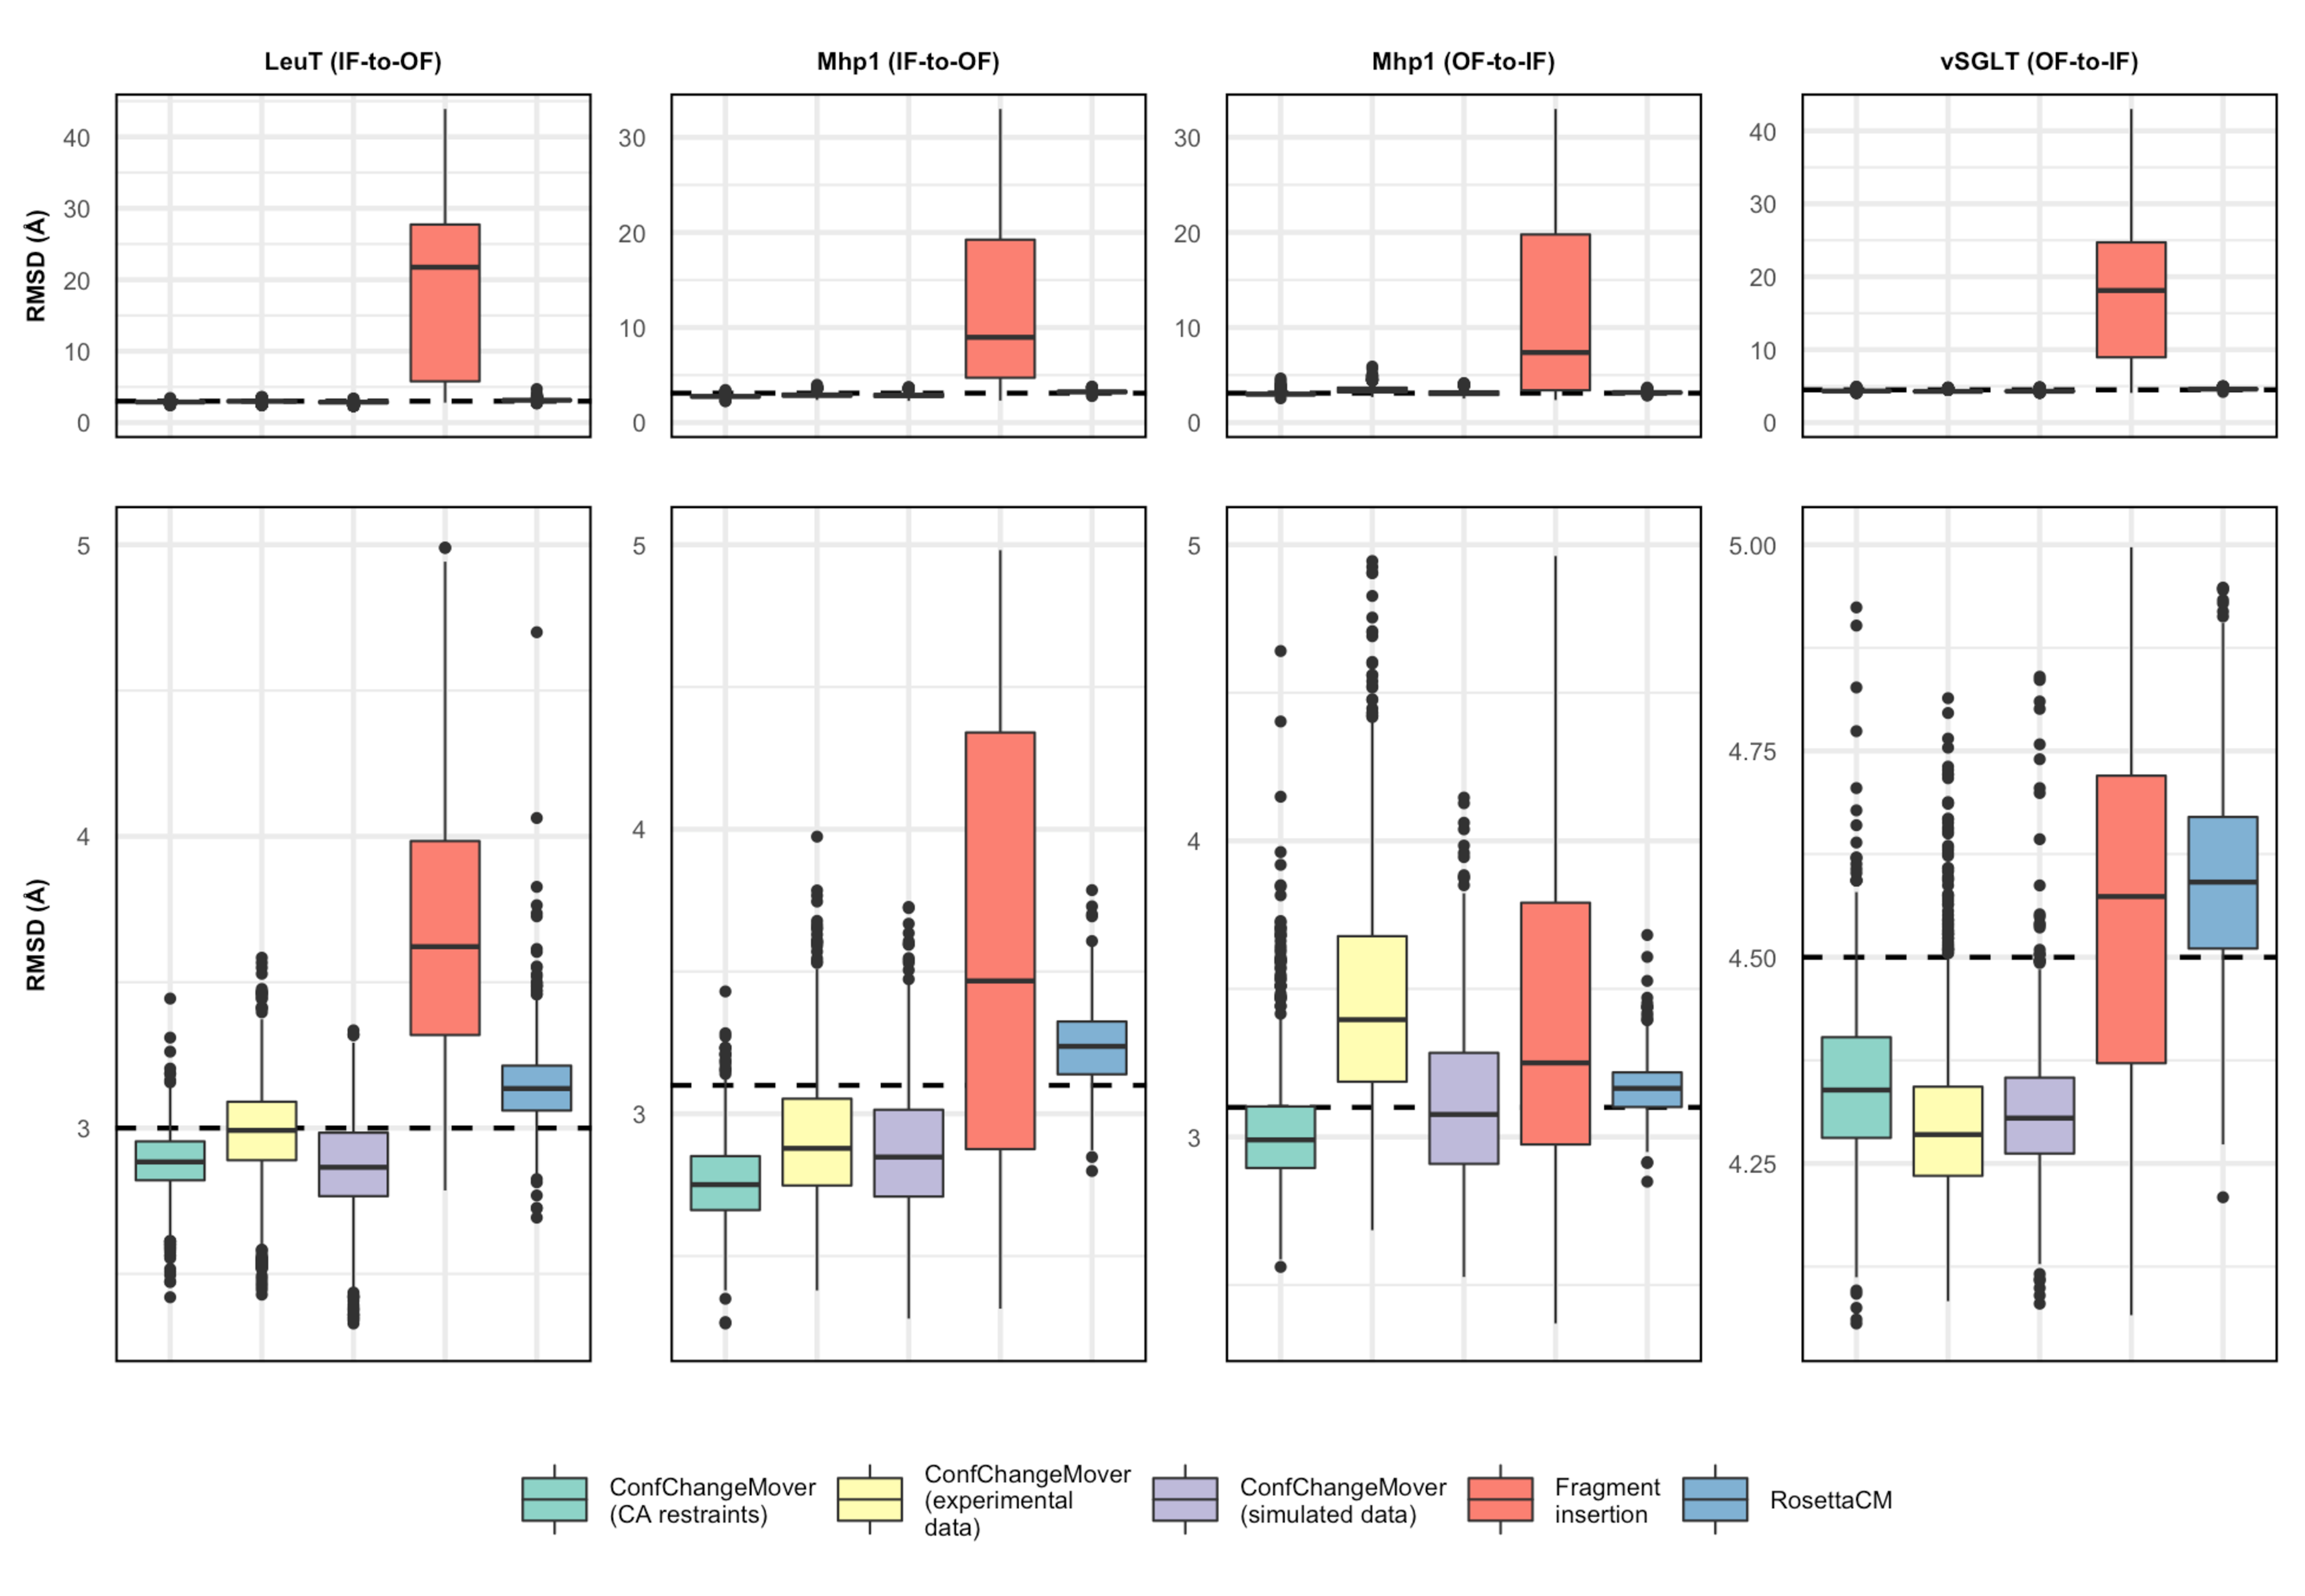
\includegraphics[width=6.5in]{Figures/ccm_leut.pdf}
 \caption[ConfChangeMover outperforms available methods in Rosetta when modeling conformational changes in LeuT-fold transporters using EPR data.]{ConfChangeMover outperforms available methods in Rosetta when modeling conformational changes in LeuT-fold transporters using EPR data. Starting models indicated by the dashed black line.}
\label{fig:ccm_leut}
\end{figure}

The results are shown in Figure \ref{fig:ccm_leut} and repeat the pattern observed in those obtained in the soluble protein benchmark. ConfChangeMover largely samples structures similar to the starting model, with virtually all models improving in \gls{rmsd} relative to the starting structure. The exception, \gls{of}-to-\gls{if} Mhp1, saw most models get worse in quality. The striking different between models generated using simulated and experimental data suggested that poor model quality could be attributed to differences between predicted and experimental spin label distances. Indeed, a distance restraint between \gls{tmh}1a and \gls{tmh}9 on the intracellular side of the protein (30/338) differed from predictions obtained using MDDS by \SI{14}{\angstrom} \citep*{Kazmier2014}. Additionally, visual examination of representative models obtained using simulated \gls{deer} restraints revealed that the kinked \gls{tmh}5 facilitating substrate egress into the cytoplasm could not be recapitulated using this method (Figure \ref{fig:ccm_bestmodels}). 

Related to this observation, we found that in three cases the $\mathrm{C_{\upalpha}}$-$\mathrm{C_{\upalpha}}$ distance restraints provided the greatest benefit, suggesting that the precision obtained when directly restraining the backbone is generally superior to those obtained from spin probes measured using \gls{deer}. The results from the fourth case, vSGLT, were not statistically different from either experimental or simulated \gls{deer} data (unpaired two-tailed $t$-test), highlighting the consistency of that crystal structure with the experimental \gls{deer} data.

\begin{figure}[h!]
\centering
\includegraphics[width=6.5in]{Figures/ccm_bestmodels.pdf}
 \caption[Lowest RMSD models obtained using ConfChangeMover with experimental EPR restraints.]{Lowest RMSD models obtained using ConfChangeMover with experimental EPR restraints.}
\label{fig:ccm_bestmodels}
\end{figure}

In marked contrast, and as was seen in the soluble protein benchmark, we found that fragment insertion similarly unfolded these models, with average \gls{rmsd} values of \SIrange{10}{25}{\angstrom} (Figure \ref{fig:ccm_soluble}). Unlike the soluble protein benchmark, in no cases did it outperform ConfChangeMover among proteins with this topology. Additionally, the homology modeling program RosettaCM sampled too conservatively and did not allow models to be modified away from the starting structure.

\subsection{Concluding remarks}

The modeling protocol ConfChangeMover is presented and discussed. Benchmarks in both soluble proteins using simulated distance restraints and membrane transporter proteins using experimental restraints show how this method can tackle various modes of conformational interconversion while generating models that nonetheless resemble the starting conformation. Its implementation as a Mover in Rosetta allows it to be used in combination with countless other modeling methods. Further development should focus on combining ConfChangeMover with other protocols, or embedding it in more complex modeling approaches \citep*{Park2018}.

\subsection{Acknowledgements}

We would like to thank Dr. Davide Sala for collaborating on this project and Dr. Marion F. Sauer for fruitful discussions during its early stages. The research in this Appendix was supported by the National Institutes of Health (R01 GM080403 and R01 GM073151), and by the Deutsche Forschungsgemeinschaft (DFG, German Research Foundation) through SFB1423, project number 421152132, subproject A07 and Z04. 